\chapter{Plasticité neuronale, apprentissage et mémoire}\label{ch:b3:learning-memory}

En 1953 un chirurgien retira la partie interne des deux lobes temporaux
d'un jeune homme atteint d'une épilepsie rebelle. Les crises se
calmèrent~; le patient, connu pendant cinquante ans sous les initiales
H.M., ne forma plus jamais le moindre souvenir durable d'un événement.
Il pouvait tenir une conversation, apprenait à suivre une étoile dans un
miroir aussi bien que quiconque --- et niait chaque jour avoir jamais vu
la tâche --- et il se rappelait son enfance. La mémoire, on le découvrit
ainsi, n'était pas une seule chose, et la fabrication de nouveaux
souvenirs d'événements dépendait d'une structure grosse comme un pouce.
Ce qui change dans un cerveau qui apprend est la plus vieille question
des neurosciences, et sa réponse, élaborée chez une limace de mer de
vingt mille neurones et dans des tranches d'\omterm{def:b3:learning-memory:kinds}{hippocampe} de rat, est que
les synapses changent de force selon ce qui les traverse --- une règle
que Donald Hebb devina en 1949 et qu'une molécule, le \omterm{prop:b3:learning-memory:nmda}{récepteur NMDA},
s'est trouvée mettre en œuvre. Ce chapitre traite de cette règle et de
sa machinerie, des circuits qui s'en servent pour stocker des lieux et
des événements, des mathématiques qui disent ce qu'un tel système peut
apprendre et combien il peut retenir, et du signal de récompense qui lui
dit ce qui mérite d'être appris.

\section{Les sortes de mémoire et où elles logent}

\begin{definition}[Formes d'apprentissage et de mémoire]\label{def:b3:learning-memory:kinds}
\index{habituation}\index{sensibilisation}\index{conditionnement}\index{mémoire déclarative}\index{mémoire procédurale}\index{consolidation}\index{hippocampe}
L'apprentissage le plus simple est \emph{non associatif}~:
l'\emph{habituation}, réponse déclinante à un stimulus inoffensif
répété, et la \emph{sensibilisation}, réponse renforcée après un
stimulus nuisible. L'apprentissage \emph{associatif} lie deux
événements~: dans le \emph{conditionnement classique} (Pavlov) un
stimulus neutre qui annonce une récompense ou une punition finit par
provoquer la réponse~; dans le \emph{conditionnement opérant} une action
récompensée est répétée. La mémoire humaine se divise en mémoire
\emph{déclarative} --- faits et événements, rappelés consciemment,
dépendant de l'\emph{hippocampe} et du lobe temporal médian --- et en
mémoire \emph{non déclarative} --- savoir-faire et habitudes (striatum,
\omterm{def:b3:nervous-systems:plan}{cervelet}), peur conditionnée (amygdale), amorçage (cortex) ---
exprimée dans la performance sans souvenir. Un souvenir est d'abord
tenu sous une forme labile à court terme, qui dure de quelques secondes
à quelques heures, et se \emph{consolide} en quelques heures à quelques
années en une forme stable à long terme qui n'a plus besoin de
l'hippocampe et réside dans le cortex.
\end{definition}

\begin{proof}[Faits expérimentaux]
Scoville et Milner (1957) rapportèrent le cas de H.M.~: après ablation
des deux \omterm{def:b3:learning-memory:kinds}{hippocampes} et du cortex voisin, son intelligence et ses
souvenirs d'avant l'opération étaient largement intacts, sa mémoire de
travail normale tant qu'il prêtait attention à quelque chose, mais il ne
pouvait plus former aucun souvenir d'un événement ni d'un fait. Il
apprenait des savoir-faire moteurs à un rythme normal au fil des jours
tout en niant s'être exercé --- la mémoire des savoir-faire n'avait donc
pas besoin de l'\omterm{def:b3:learning-memory:kinds}{hippocampe} --- et il se rappelait mieux le passé
lointain que les années précédant l'opération, de sorte que l'\omterm{def:b3:learning-memory:kinds}{hippocampe}
était nécessaire pour déposer et pour tenir un temps les souvenirs
déclaratifs, non pour les stocker à jamais. Des singes et des rats à
lésions comparables montrèrent la même dissociation, et l'étude d'un
seul patient réorganisa le domaine.
\end{proof}

\section{La règle de Hebb et sa molécule}

\begin{definition}[Plasticité hebbienne, PLT et DLT]\label{def:b3:learning-memory:ltp}
\index{règle de Hebb}\index{potentialisation à long terme}\index{dépression à long terme}\index{plasticité dépendante du temps des potentiels}
Hebb (1949) proposa que, lorsqu'un neurone présynaptique participe à
plusieurs reprises à la décharge d'un neurone postsynaptique, la
connexion entre eux se renforce --- «~les cellules qui déchargent
ensemble se câblent ensemble~». La \emph{potentialisation à long terme}
(PLT) en est la forme expérimentale~: une brève bouffée de stimulation à
haute fréquence d'une voie laisse plus fortes, des heures durant dans
une tranche et des semaines durant chez l'animal, les synapses qu'elle a
activées. La PLT est \emph{spécifique de l'entrée} (seules les synapses
stimulées changent), \emph{associative} (une entrée faible appariée à
une forte vers la même cellule est potentialisée) et demande une
\emph{\omterm{def:b3:structural-biology:allostery}{coopérativité}} entre entrées pour dépolariser la cellule. La
\emph{dépression à long terme} (DLT) en est l'inverse, produite par une
activité prolongée à basse fréquence. Dans la \emph{plasticité
dépendante du temps des potentiels} le signe est fixé par l'ordre~: un
potentiel présynaptique quelques millisecondes \emph{avant} le
postsynaptique renforce la synapse, un potentiel juste \emph{après}
l'affaiblit, dans une fenêtre d'environ \qty{20}{ms} de part et d'autre
--- de sorte qu'une synapse apprend à prédire, et non seulement à
corréler.
\end{definition}

\begin{proposition}[Le récepteur NMDA comme détecteur de coïncidence]\label{prop:b3:learning-memory:nmda}
\index{récepteur NMDA}\index{récepteur AMPA}\index{CaMKII}\index{CREB}\index{épine dendritique}
Aux synapses excitatrices le glutamate agit sur deux récepteurs. Le
récepteur \emph{AMPA} s'ouvre à la liaison et porte le courant
synaptique ordinaire. Le récepteur \emph{NMDA} lie le glutamate mais est
bloqué au potentiel de repos par un ion magnésium logé dans son pore~;
ce n'est que lorsque la membrane postsynaptique est dépolarisée --- par
de nombreuses entrées à la fois, ou par un potentiel d'action qui
rétropropage --- que le magnésium est expulsé et que le canal conduit,
laissant entrer du calcium. Le \omterm{prop:b3:learning-memory:nmda}{récepteur NMDA} ne s'ouvre donc que
lorsque la libération présynaptique (le glutamate) coïncide avec
l'activité postsynaptique (la dépolarisation)~: c'est la porte «~et~» de
Hebb dans une seule protéine. Le calcium qui entre dans une \emph{\omterm{prop:b3:learning-memory:nmda}{épine
dendritique}} active la kinase \emph{CaMKII}, qui phosphoryle les
\omterm{prop:b3:learning-memory:nmda}{récepteurs AMPA} et en fait venir davantage dans la synapse depuis une
réserve --- la synapse est plus forte en quelques minutes (PLT précoce).
Une montée de calcium ample et lente active au contraire la phosphatase
calcineurine, qui retire des \omterm{prop:b3:learning-memory:nmda}{récepteurs AMPA}~: c'est la DLT. Une
potentialisation qui dure plus de quelques heures (PLT tardive) exige de
nouvelles protéines~: des kinases gagnent le noyau, le facteur de
transcription \emph{CREB} allume des gènes, et l'épine grandit et peut
se diviser --- la même exigence d'expression génique qui sépare la
mémoire à court terme de la mémoire à long terme chez tous les animaux
étudiés.
\end{proposition}

\begin{proof}[Faits expérimentaux]
Bliss et L\o mo (1973) stimulèrent la voie perforante de l'\omterm{def:b3:learning-memory:kinds}{hippocampe} du
lapin par un train d'impulsions et trouvèrent la réponse évoquée
agrandie pendant des heures --- la première PLT. Collingridge (1983)
montra qu'un bloqueur du \omterm{prop:b3:learning-memory:nmda}{récepteur NMDA} (l'AP5) empêchait l'induction de
la PLT mais non la réponse synaptique ordinaire~; Morris (1986) infusa
de l'AP5 dans l'\omterm{def:b3:learning-memory:kinds}{hippocampe} de rats et constata qu'ils ne pouvaient plus
apprendre la position d'une plate-forme cachée dans un bassin d'eau
tout en nageant et en voyant normalement~; et des souris chez qui le
\omterm{prop:b3:learning-memory:nmda}{récepteur NMDA} n'était supprimé que dans la région \omterm{def:b3:learning-memory:hippocampus}{CA1} de l'\omterm{def:b3:learning-memory:kinds}{hippocampe}
manquaient à la fois de PLT là et de mémoire spatiale. Le même
récepteur, au même endroit, était nécessaire au changement synaptique et
à l'apprentissage.
\end{proof}

\begin{omfigure}
\begin{tikzpicture}[every node/.style={font=\scriptsize}, >=stealth]
  % presynaptic terminal
  \draw[thick, omDef, fill=omDef!12] (0,2.2) .. controls (0,3.4) and (4,3.4) .. (4,2.2) -- (4,1.7) -- (0,1.7) -- cycle;
  \node at (2,2.8) {terminaison présynaptique};
  \foreach \p in {(0.8,2.0),(1.6,2.1),(2.6,2.0),(3.3,2.1)} \draw[thick, fill=omDef!40] \p circle (0.17);
  \foreach \p in {(1.2,1.45),(2.0,1.5),(2.9,1.42)} \fill[omProp] \p circle (0.06);
  \node[right, omProp] at (3.3,1.45) {glutamate};
  % postsynaptic spine
  \draw[thick, omMeth!70!black, fill=omMeth!10] (-0.6,1.1) -- (4.4,1.1) -- (4.4,-1.2) -- (-0.6,-1.2) -- cycle;
  \node at (0.6,-0.9) {épine dendritique};
  % AMPA
  \draw[thick, fill=omMeth!45] (0.2,0.85) rectangle (0.6,1.35); \node[below, align=center] at (0.1,0.8) {AMPA~:\\Na$^{+}$ entre};
  \draw[->, thick] (0.4,1.7) -- (0.4,0.95);
  % NMDA with Mg
  \draw[thick, fill=omThm!35] (2.4,0.85) rectangle (2.9,1.35); \fill[gray!70] (2.65,1.1) circle (0.09); \node[right, font=\tiny] at (2.95,1.1) {blocage par Mg$^{2+}$};
  \node[below, align=center] at (2.65,0.8) {NMDA~: exige le glutamate\\\emph{et} la dépolarisation};
  \draw[->, thick, omThm] (2.65,0.15) -- (2.65,-0.5) node[below] {Ca$^{2+}$};
  % downstream
  \node[draw, rounded corners, fill=omThm!15, font=\tiny] (cam) at (5.6,0.3) {CaMKII};
  \draw[->, thick] (2.9,-0.5) -- (cam);
  \node[draw, rounded corners, fill=omMeth!25, font=\tiny, align=center] (ampa) at (8.2,1.0) {plus de récepteurs AMPA\\insérés~: PLT précoce (minutes)};
  \node[draw, rounded corners, fill=omMeth!25, font=\tiny, align=center] (creb) at (8.2,-0.5) {CREB, protéines nouvelles,\\croissance de l'épine~: PLT tardive (heures et plus)};
  \draw[->, thick] (cam) -- (ampa.west); \draw[->, thick] (cam) -- (creb.west);
  \node[draw, rounded corners, fill=omDef!15, font=\tiny, align=center] (ltd) at (8.2,-1.8) {Ca$^{2+}$ lent et faible~: calcineurine,\\AMPA retirés~: DLT};
  \draw[->, thick, dashed] (2.9,-0.7) .. controls (4.5,-1.6) .. (ltd.west);
\end{tikzpicture}

{\small Le \omterm{prop:b3:learning-memory:nmda}{récepteur NMDA} comme porte de Hebb. Le glutamate seul ouvre
les \omterm{prop:b3:learning-memory:nmda}{récepteurs AMPA}~; le canal NMDA ne conduit que si l'épine est aussi
dépolarisée et que son magnésium s'en va. Le calcium qui entre alors
fixe l'avenir de la synapse~: une montée rapide et ample la renforce,
une montée lente et faible l'affaiblit.}
\end{omfigure}

\begin{omfigure}
\begin{tikzpicture}
\begin{axis}[
  width=6.6cm, height=5.2cm,
  axis x line=bottom, axis y line=left,
  xmin=-20, xmax=120, ymin=0, ymax=220,
  xlabel={minutes}, ylabel={réponse synaptique (\%)},
  xlabel style={font=\small, at={(axis description cs:0.5,-0.12)}, anchor=north}, ylabel style={font=\small},
  tick label style={font=\scriptsize}, xtick={0,30,60,90,120}, ytick={0,100,200},
  clip=false,
]
\addplot[only marks, mark=*, mark size=1pt, omDef] coordinates {(-18,100) (-15,98) (-12,102) (-9,99) (-6,101) (-3,100) (2,195) (5,180) (8,172) (11,168) (15,165) (20,162) (30,160) (40,158) (50,157) (60,156) (70,156) (80,155) (90,155) (100,154) (110,154) (120,154)};
\addplot[only marks, mark=o, mark size=1pt, gray] coordinates {(-18,100) (-12,101) (-6,99) (2,102) (8,100) (15,101) (30,100) (45,99) (60,101) (75,100) (90,100) (105,101) (120,100)};
\draw[->, thick, omThm] (axis cs:0,215) -- (axis cs:0,200); \node[font=\scriptsize, omThm, anchor=south] at (axis cs:0,216) {tétanos};
\node[font=\scriptsize, omDef, anchor=south west] at (axis cs:35,168) {voie stimulée~: PLT};
\node[font=\scriptsize, gray, anchor=north west] at (axis cs:35,95) {voie témoin~: inchangée};
\end{axis}
\begin{axis}[
  at={(7.6cm,0)}, anchor=south west,
  width=6.6cm, height=5.2cm,
  axis x line=middle, axis y line=middle,
  xmin=-60, xmax=60, ymin=-60, ymax=100,
  xlabel={$t_{\text{pré}} - t_{\text{post}}$ (ms)}, ylabel={$\Delta w$ (\%)},
  xlabel style={font=\small, at={(axis description cs:0.5,-0.06)}, anchor=north}, ylabel style={font=\small, at={(axis description cs:0.5,1.02)}, anchor=south},
  tick label style={font=\scriptsize}, xtick={-40,-20,20,40}, ytick={-40,40,80},
  clip=false,
]
\addplot[very thick, omMeth!70!black, domain=-60:-0.5, samples=60] {80*exp(x/15)};
\addplot[very thick, omThm, domain=0.5:60, samples=60] {-45*exp(-x/25)};
\node[font=\scriptsize, omMeth!70!black, anchor=south east] at (axis cs:-8,62) {pré avant post~: PLT};
\node[font=\scriptsize, omThm, anchor=north west] at (axis cs:8,-22) {post avant pré~: DLT};
\end{axis}
\end{tikzpicture}

{\small À gauche~: la \omterm{def:b3:learning-memory:ltp}{potentialisation à long terme} --- après un bref
tétanos la réponse de la voie stimulée reste agrandie des heures durant
tandis qu'une voie non stimulée vers les mêmes cellules est inchangée
(la spécificité d'entrée). À droite~: la fenêtre temporelle --- la
synapse se renforce si le potentiel présynaptique précède et s'affaiblit
s'il suit.}
\end{omfigure}

\begin{theorem}[Ce qu'apprend une synapse hebbienne]\label{thm:b3:learning-memory:hebb}
\index{apprentissage hebbien!composante principale}\index{règle d'Oja}
Soit un neurone qui reçoit des entrées
$\mathbf{x} = (x_{1},\dots,x_{n})$ par des poids $\mathbf{w}$ et répond
linéairement, $y = \mathbf{w}\cdot\mathbf{x}$. La \omterm{def:b3:learning-memory:ltp}{règle de Hebb},
$\Delta\mathbf{w} = \eta\, y\,\mathbf{x}$, donne en moyenne sur les
entrées
\[
\langle\Delta\mathbf{w}\rangle = \eta\,C\,\mathbf{w}, \qquad C =
\langle\mathbf{x}\mathbf{x}^{\mathsf{T}}\rangle ,
\]
où $C$ est la matrice de corrélation des entrées. Les poids croissent
sans borne, et croissent le plus vite le long du vecteur propre de $C$
de plus grande valeur propre~: la synapse en vient à détecter le motif
d'entrée le plus souvent présent --- la \emph{composante principale} de
ses entrées. Avec un terme qui pénalise les grands poids, la
\emph{\omterm{thm:b3:learning-memory:hebb}{règle d'Oja}}
$\Delta\mathbf{w} = \eta\, y\,(\mathbf{x} - y\,\mathbf{w})$, le
vecteur des poids converge vers ce vecteur propre
normalisé à la longueur un, et le neurone devient un détecteur stable de
la corrélation dominante de ce qu'il voit.
\end{theorem}
\begin{proof}
En portant $y = \mathbf{w}\cdot\mathbf{x} = \mathbf{x}^{\mathsf{T}}
\mathbf{w}$ dans la \omterm{def:b3:learning-memory:ltp}{règle de Hebb} on obtient $\Delta\mathbf{w} = \eta\,\mathbf{x}
\mathbf{x}^{\mathsf{T}}\mathbf{w}$, dont la moyenne sur les entrées (avec
$\mathbf{w}$ qui change lentement) vaut $\eta C\mathbf{w}$. $C$ est symétrique
et semi-définie positive, donc elle a des vecteurs propres orthogonaux $\mathbf{e}_{k}$
de valeurs propres $\lambda_{k} \ge 0$~; en écrivant $\mathbf{w} = \sum_{k}
a_{k}\mathbf{e}_{k}$, chaque composante obéit à $\Delta a_{k} = \eta\lambda_{k}
a_{k}$ et croît comme $(1 + \eta\lambda_{k})^{t}$, de sorte que la
composante de plus grande valeur propre en vient à dominer la direction
de $\mathbf{w}$ tandis que sa longueur diverge. La \omterm{thm:b3:learning-memory:hebb}{règle d'Oja} a pour
moyenne $\eta(C\mathbf{w} -
(\mathbf{w}^{\mathsf{T}}C\mathbf{w})\mathbf{w})$~; en un point fixe
$C\mathbf{w} = (\mathbf{w}^{\mathsf{T}}C\mathbf{w})\mathbf{w}$, donc
$\mathbf{w}$ est un vecteur propre avec $\lambda = \mathbf{w}^{\mathsf{T}}
C\mathbf{w} = \lambda|\mathbf{w}|^{2}$, d'où $|\mathbf{w}| = 1$~; le point
fixe le long de la plus grande valeur propre est le point stable (une
perturbation vers un autre vecteur propre se réduit, puisque la valeur
propre de celui-ci est plus petite), ce qui est admis ici.
\end{proof}

\begin{example}[Deux entrées]\label{ex:b3:learning-memory:two-inputs}
Un neurone reçoit deux entrées qui sont d'ordinaire actives ensemble, de
sorte que $C =
\begin{pmatrix} 1 & 0.8 \\ 0.8 & 1\end{pmatrix}$. Les vecteurs propres
sont $(1,1)/\sqrt{2}$ de valeur propre $1.8$ et $(1,-1)/\sqrt{2}$ de
valeur propre $0.2$. En partant de $\mathbf{w} = (1, 0)$, la \omterm{def:b3:learning-memory:ltp}{règle de
Hebb} tourne $\mathbf{w}$ vers $(1,1)$ après beaucoup de petits pas~: le
neurone apprend à répondre aux deux entrées \emph{ensemble}, et à
ignorer les rares occasions où une seule décharge --- il a extrait la
corrélation. Avec la \omterm{thm:b3:learning-memory:hebb}{règle d'Oja} les poids se fixent à $(0.71, 0.71)$.
C'est en ce sens que les synapses hebbiennes apprennent ce qui va
ensemble, et c'est pourquoi la propriété associative de la PLT, qui
apparie une entrée faible à une forte, découle de la règle.
\end{example}

\section{Une limace qui apprend}

\begin{proposition}[La sensibilisation chez l'\emph{Aplysia}]\label{prop:b3:learning-memory:aplysia}
\index{Aplysia}\index{facilitation présynaptique}\index{AMPc}\index{PKA}
La limace de mer \emph{Aplysia} rétracte sa branchie quand on touche son
siphon, réflexe de quelques dizaines de neurones identifiables. Un choc
sur la queue la \emph{sensibilise}~: la rétraction à un toucher léger
est renforcée, pendant des minutes après un choc et pendant des semaines
après plusieurs. Kandel et ses collègues (des années 1970 aux années
1990) ont rapporté le changement à la synapse entre le neurone sensoriel
du siphon et le motoneurone de la branchie. Le choc sur la queue excite
un \omterm{def:b3:nervous-systems:cells}{interneurone} qui libère de la sérotonine sur la terminaison du
neurone sensoriel~; la sérotonine élève l'AMP cyclique, qui active la
protéine kinase A, qui phosphoryle et ferme un canal potassique~; les
potentiels d'action de la terminaison s'élargissent, plus de calcium
entre, et plus de transmetteur est libéré par potentiel --- la
\emph{\omterm{prop:b3:learning-memory:aplysia}{facilitation présynaptique}}, changement covalent qui dure des
minutes. Des chocs répétés envoient la kinase au noyau, où elle active
CREB, qui allume des gènes qui bâtissent de nouvelles terminaisons
synaptiques~: la mémoire à long terme est faite de synapses
supplémentaires, et elle est bloquée par des inhibiteurs de la synthèse
protéique donnés pendant l'entraînement mais non après.
L'\emph{\omterm{def:b3:learning-memory:kinds}{habituation}} est l'inverse, une dépression de la même synapse~;
et le \emph{\omterm{def:b3:learning-memory:kinds}{conditionnement} classique}, qui apparie le toucher au choc,
renforce la facilitation aux synapses qui étaient actives juste avant
l'arrivée de la sérotonine --- une coïncidence hebbienne mise en œuvre
du côté présynaptique, par une adénylate cyclase que stimulent ensemble
le calcium et la sérotonine.
\end{proposition}

\begin{omfigure}
\begin{tikzpicture}[every node/.style={font=\scriptsize}, >=stealth]
  \node[draw, thick, rounded corners, fill=omDef!20, minimum width=2cm] (sn) at (0,0) {neurone sensoriel du siphon};
  \node[draw, thick, rounded corners, fill=omMeth!25, minimum width=2cm] (mn) at (6.2,0) {motoneurone de la branchie};
  \node[draw, thick, rounded corners, fill=omProp!30, align=center] (in) at (2.8,2.4) {interneurone facilitateur\\(sérotonine)};
  \node[left] at (-2.1,0) {toucher}; \draw[->, thick] (-2.0,0) -- (sn);
  \draw[->, very thick] (sn) -- (mn) node[pos=0.45, below, align=center, font=\tiny] {la synapse\\qui change};
  \draw[->, thick] (mn) -- (8.4,0) node[right] {la branchie se rétracte};
  \node[above] at (2.8,3.1) {choc sur la queue}; \draw[->, thick] (2.8,3.05) -- (in);
  \draw[->, thick, omProp] (in) -- (2.8,0.25);
  \node[right, align=left, font=\tiny] at (6.6,1.6) {sérotonine $\to$ AMPc $\to$ PKA $\to$ canal K$^{+}$ fermé\\$\to$ potentiel élargi, plus de Ca$^{2+}$,\\plus de transmetteur (minutes)~;\\répété~: PKA $\to$ CREB $\to$ terminaisons nouvelles};
\end{tikzpicture}

{\small Le circuit de la \omterm{def:b3:learning-memory:kinds}{sensibilisation} chez l'\emph{Aplysia}. La
sérotonine venue d'un \omterm{def:b3:nervous-systems:cells}{interneurone} agit sur la terminaison sensorielle,
et la même synapse porte la mémoire à court terme sous forme d'un canal
phosphorylé et la mémoire à long terme sous forme de terminaisons
nouvelles.}
\end{omfigure}

\begin{omfigure}
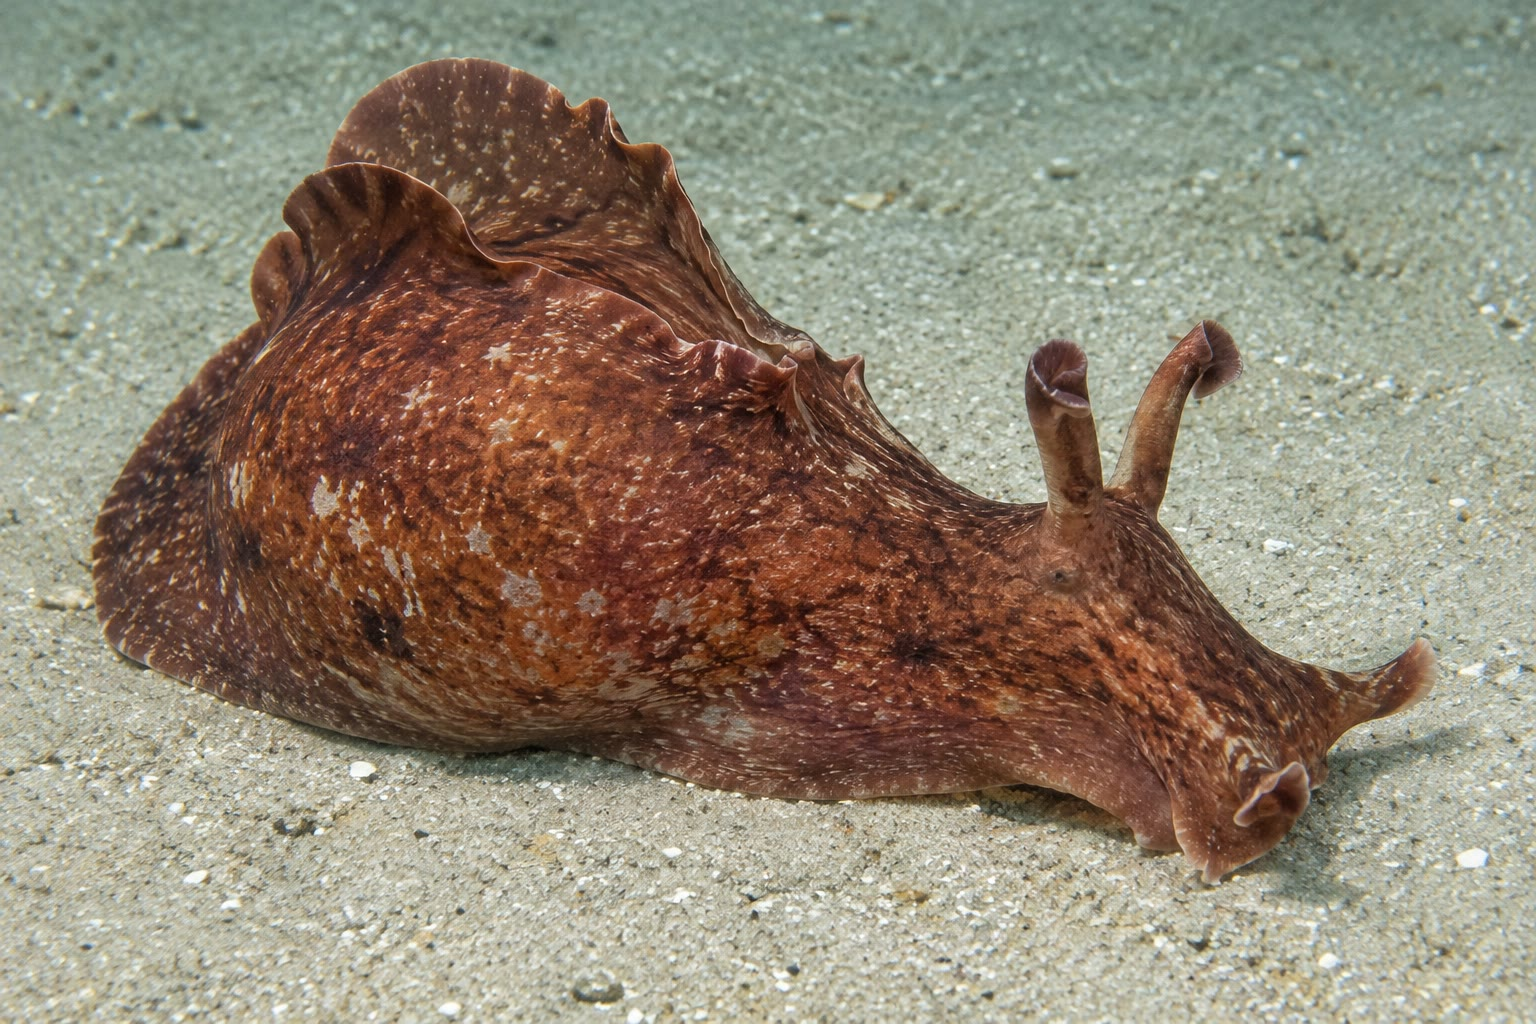
\includegraphics[width=0.46\linewidth]{images/book5/ai/b5-19-aplysia.jpg}\hspace{0.04\linewidth}
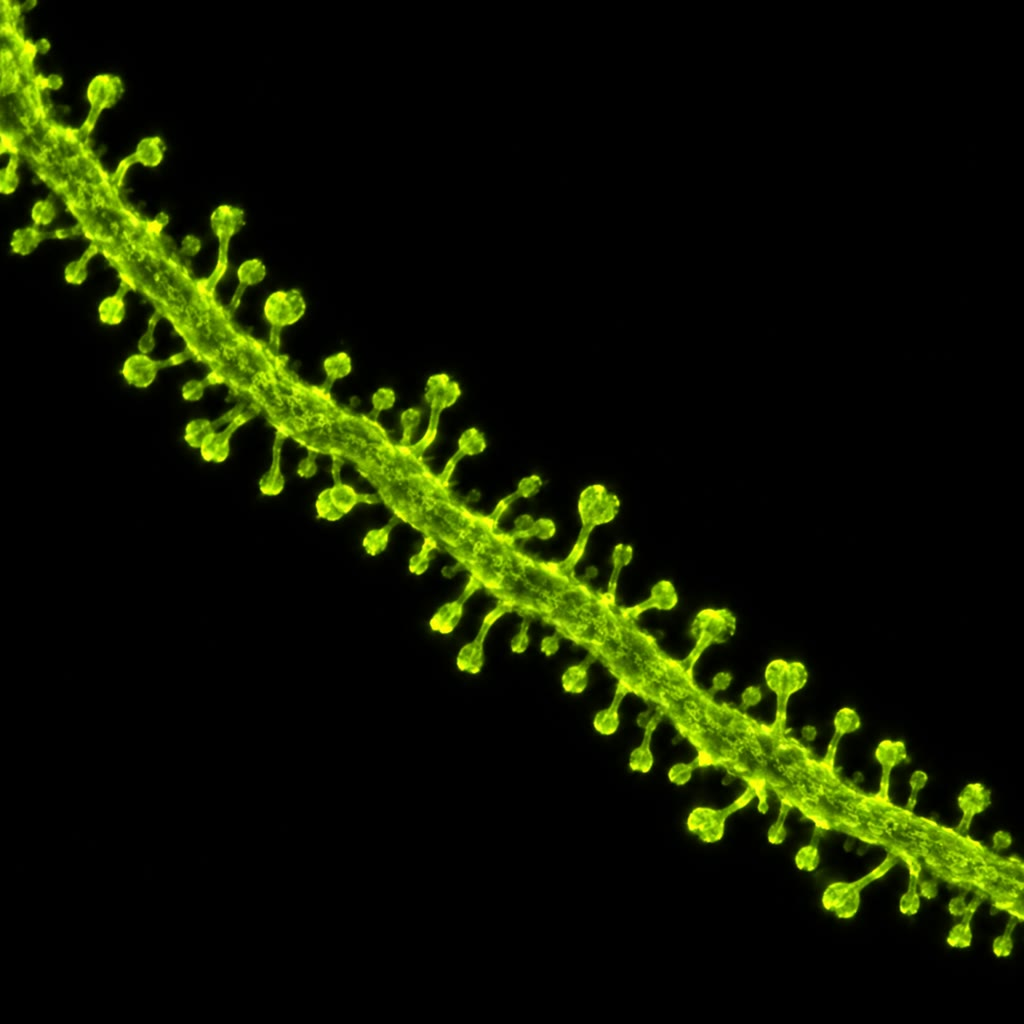
\includegraphics[width=0.36\linewidth]{images/book5/ai/b5-19-dendritic-spines.jpg}

{\small À gauche~: \emph{Aplysia californica}, dont les neurones peu
nombreux et gros permettent de trouver et d'enregistrer la synapse d'un
souvenir. À droite~: une dendrite hérissée d'épines, chacune le versant
postsynaptique d'une synapse excitatrice et chacune un compartiment dont
le calcium décide de son propre sort.}
\end{omfigure}

\section{Des circuits pour les lieux et les événements}

\begin{definition}[Le circuit hippocampique]\label{def:b3:learning-memory:hippocampus}
\index{gyrus denté}\index{CA3}\index{CA1}\index{cellule de lieu}\index{cellule de grille}\index{complétion de motif}\index{rejeu}
L'entrée corticale gagne l'\omterm{def:b3:learning-memory:kinds}{hippocampe} par le cortex entorhinal et
traverse trois étages~: le \emph{gyrus denté}, dont les cellules
granulaires sont plus nombreuses que leurs entrées et déchargent
parcimonieusement (ce qui sépare les motifs semblables)~; \emph{CA3},
dont les cellules pyramidales sont connectées récurremment les unes aux
autres, chacune recevant des milliers de synapses des autres --- un
réseau \emph{autoassociatif} qui sait compléter un motif stocké à partir
d'un fragment~; et \emph{CA1}, qui compare la sortie de CA3 à l'entrée
directe et renvoie le résultat au cortex. Chez un rat qui explore une
arène, une cellule pyramidale de l'\omterm{def:b3:learning-memory:kinds}{hippocampe} ne décharge que lorsque
l'animal est à un endroit --- une \emph{cellule de lieu} (O'Keefe, 1971)
--- et quelques centaines d'entre elles cartographient l'arène~; en
amont, dans le cortex entorhinal, les \emph{cellules de grille} (Moser,
2005) déchargent aux sommets d'un réseau hexagonal qui couvre l'espace,
système de coordonnées à partir duquel se construisent les champs de
lieu. Pendant le sommeil et le repos les séquences de cellules de lieu
qui ont déchargé pendant un parcours sont \emph{rejouées} à grande
vitesse, et bloquer le rejeu abîme le souvenir du parcours~: l'\omterm{def:b3:learning-memory:kinds}{hippocampe}
répète au cortex les chemins de la journée.
\end{definition}

\begin{omfigure}
\begin{tikzpicture}[every node/.style={font=\scriptsize}, >=stealth]
  % trisynaptic loop
  \node[draw, thick, rounded corners, fill=gray!15, align=center] (ec) at (0,0) {cortex entorhinal\\(cellules de grille)};
  \node[draw, thick, rounded corners, fill=omDef!20, align=center] (dg) at (3.2,1.4) {gyrus denté~:\\séparation des motifs};
  \node[draw, thick, rounded corners, fill=omProp!30, align=center] (ca3) at (7.2,1.4) {CA3, récurrent~:\\complétion des motifs};
  \node[draw, thick, rounded corners, fill=omMeth!25, align=center] (ca1) at (7.2,-1.4) {CA1~:\\compare, envoie};
  \draw[->, thick] (ec) -- (dg); \draw[->, thick] (dg) -- (ca3); \draw[->, thick] (ca3) -- (ca1); \draw[->, thick] (ca1) -- (ec) node[pos=0.3, below, sloped, font=\tiny] {retour au cortex};
  \draw[->, thick, dashed] (ec) -- (ca1.north west) node[pos=0.7, above, sloped, font=\tiny] {voie directe};
  \draw[->, thick, omProp!80!black] (ca3.north) .. controls (6.6,2.6) and (7.8,2.6) .. (ca3.north east) node[pos=0.5, above, font=\tiny] {collatérales récurrentes};
  % place field map
  \begin{scope}[xshift=10.4cm, yshift=-0.2cm]
    \draw[thick] (0,0) rectangle (3,2.4); \node[below] at (1.5,-0.05) {l'arène, vue de dessus};
    \foreach \p/\c in {(0.7,1.8)/omThm, (2.1,1.9)/omDef, (1.4,0.9)/omMeth, (2.5,0.6)/omProp} { \fill[\c!60] \p circle (0.32); \fill[\c!90] \p circle (0.16); }
    \node[above] at (1.5,2.45) {les champs de décharge de quatre cellules de lieu};
  \end{scope}
\end{tikzpicture}

{\small À gauche~: la boucle hippocampique --- séparation dans le \omterm{def:b3:learning-memory:hippocampus}{gyrus
denté}, stockage et complétion dans le \omterm{def:b3:learning-memory:hippocampus}{CA3} récurrent, comparaison dans
\omterm{def:b3:learning-memory:hippocampus}{CA1}. À droite~: chaque \omterm{def:b3:learning-memory:hippocampus}{cellule de lieu} décharge dans une région d'une
arène~; ensemble elles cartographient l'espace.}
\end{omfigure}

\begin{proposition}[Ce que retient un réseau autoassociatif]\label{prop:b3:learning-memory:capacity}
\index{réseau de Hopfield}\index{capacité mnésique}
Un réseau de $N$ neurones, chacun connecté à tous les autres avec des
poids hebbiens $w_{ij} \propto \sum_{\mu}\xi_{i}^{\mu}\xi_{j}^{\mu}$
sommés sur les motifs binaires stockés $\xi^{\mu}$, retrouve un motif
stocké à partir d'un indice altéré ou partiel en s'installant dedans
comme dans un attracteur (Hopfield, 1982). Il le fait de façon fiable
jusqu'à environ $P
\approx 0.14N$ motifs aléatoires~; au-delà les motifs interfèrent et la
récupération s'effondre. Le \omterm{def:b3:learning-memory:hippocampus}{CA3} d'un rat, avec quelque $3\times 10^{5}$
cellules pyramidales, pourrait à cette estime tenir quelque
$4\times 10^{4}$ motifs --- l'ordre de grandeur des lieux ou des
épisodes distincts qu'un animal rencontre en une saison --- et sa
décharge parcimonieuse (quelques pour cent de cellules actives dans un
motif) élève encore la capacité. La complétion d'un motif à partir d'un
indice est ce qui permet à une odeur ou à un coin de rappeler une scène
entière~; le prix est que les souvenirs semblables fusionnent, ce à quoi
résiste la séparation opérée par le \omterm{def:b3:learning-memory:hippocampus}{gyrus denté}.
\end{proposition}
\admitted

\begin{method}[Éprouver la mémoire et son mécanisme]\label{met:b3:learning-memory:tests}
\index{piscine de Morris}\index{conditionnement de peur}\index{engramme}
(1) Une tâche spatiale~: la \omterm{met:b3:learning-memory:tests}{piscine de Morris} --- un rat nage dans une
eau opaque vers une plate-forme cachée à un endroit fixe, en apprend la
position d'après les repères de la pièce au fil des jours, et on
l'éprouve par le temps passé à chercher dans le bon quadrant quand la
plate-forme est retirée~; les lésions de l'\omterm{def:b3:learning-memory:kinds}{hippocampe}, les bloqueurs
NMDA et la perte de la PLT abolissent chacun l'apprentissage. (2) Une
tâche associative~: le \omterm{met:b3:learning-memory:tests}{conditionnement de peur} --- un son apparié à un
choc sur la patte finit par provoquer l'immobilisation~; le souvenir
dépend de l'amygdale, et une version propre au contexte de
l'\omterm{def:b3:learning-memory:kinds}{hippocampe}. (3) Un test de mécanisme~: bloquer le candidat (un
médicament, une invalidation restreinte à une région et à un moment) et
montrer que l'apprentissage échoue alors que la perception et le
mouvement non. (4) L'engramme~: marquer les neurones actifs pendant
l'apprentissage avec un canal sensible à la lumière
(\cref{ch:b3:nervous-systems}) puis les réactiver plus tard par la
lumière --- l'animal s'immobilise dans un contexte sûr, comme s'il se
souvenait~; les faire taire bloque le rappel. La mémoire est dans des
cellules identifiables et leurs synapses, et on peut l'allumer et
l'éteindre.
\end{method}

\begin{omfigure}
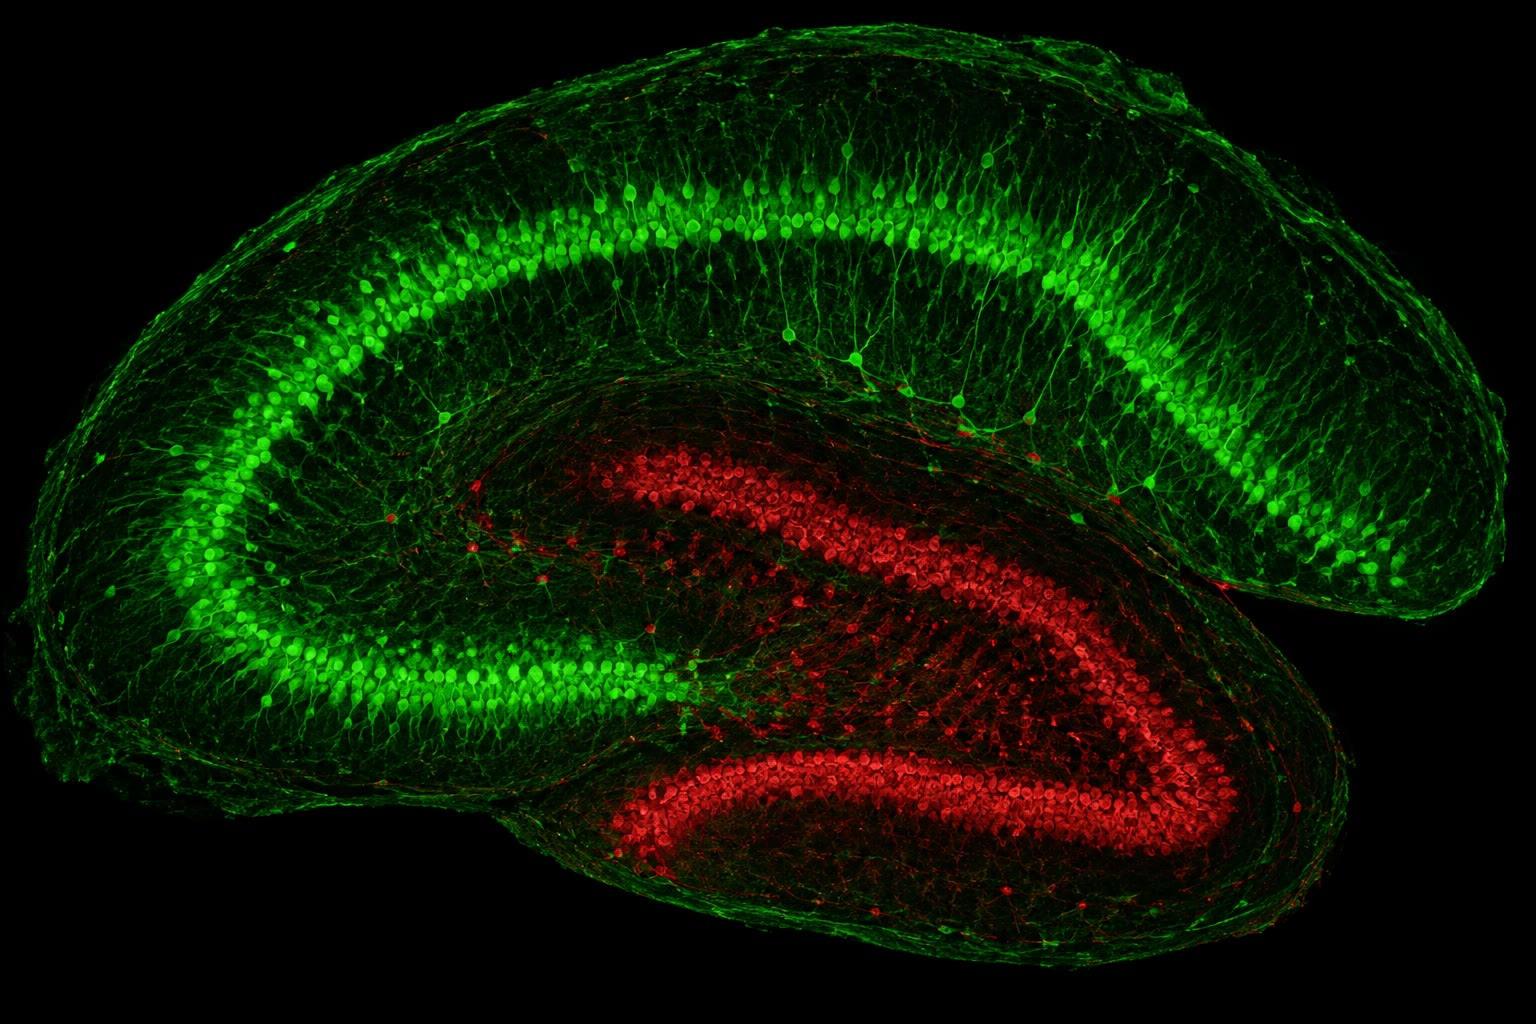
\includegraphics[width=0.56\linewidth]{images/book5/ai/b5-19-hippocampus-section.jpg}

{\small Une coupe de l'\omterm{def:b3:learning-memory:kinds}{hippocampe} d'un rongeur~: la bande incurvée de
cellules pyramidales (en vert) de \omterm{def:b3:learning-memory:hippocampus}{CA3} à \omterm{def:b3:learning-memory:hippocampus}{CA1} et le \omterm{def:b3:learning-memory:hippocampus}{gyrus denté} (en rouge)
qui s'y emboîte. Tout souvenir spatial de l'animal passe par cette
boucle.}
\end{omfigure}

\section{Récompense, prédiction et la plasticité d'une vie}

\begin{proposition}[Apprendre par l'erreur de prédiction]\label{prop:b3:learning-memory:rescorla}
\index{règle de Rescorla--Wagner}\index{erreur de prédiction}\index{dopamine}
Soit $V$ la valeur qu'un animal attache à un indice et $\lambda$ la
récompense qui le suit. La \omterm{prop:b3:learning-memory:rescorla}{règle de Rescorla--Wagner} (1972) dit qu'à
chaque essai la valeur change d'une fraction $\alpha$ de l'\emph{\omterm{prop:b3:learning-memory:rescorla}{erreur
de prédiction}}~:
\[
\Delta V = \alpha\,(\lambda - V), \qquad
V_{n} = \lambda\bigl(1 - (1-\alpha)^{n}\bigr) ,
\]
de sorte que l'apprentissage est rapide d'abord et ralentit à mesure que
la prédiction s'améliore, s'arrête quand la récompense est entièrement
prédite, et s'inverse (l'extinction) quand la récompense est retirée.
Quand deux indices sont présentés ensemble ils partagent une seule
prédiction, si bien qu'un indice qui n'ajoute rien à une prédiction déjà
faite n'est pas appris (le \emph{blocage}). Schultz (1997) enregistra
chez le singe les neurones dopaminergiques du mésencéphale et trouva
qu'ils déchargent à une récompense inattendue, se taisent à une
récompense entièrement prédite, et plongent sous leur niveau de base
quand une récompense prédite n'arrive pas~: ils diffusent
$\lambda - V$, l'\omterm{prop:b3:learning-memory:rescorla}{erreur de prédiction} elle-même, au striatum et au
cortex, où la dopamine autorise la plasticité aux synapses récemment
actives. Apprendre ce qui prédit la récompense, c'est de la plasticité
hebbienne avec un troisième facteur qui dit si l'issue a été meilleure
ou pire que prévu --- et les drogues, en poussant la dopamine
directement, contrefont un «~mieux que prévu~» permanent.
\end{proposition}
\begin{proof}
La récurrence $V_{n+1} = V_{n} + \alpha(\lambda - V_{n})$ donne
$\lambda - V_{n+1} = (1-\alpha)(\lambda - V_{n})$, de sorte que l'erreur
se réduit géométriquement, $\lambda - V_{n} = (1-\alpha)^{n}\lambda$ à
partir de $V_{0} =
0$, d'où la formule. Pour deux indices $A$ et $B$ présentés ensemble la
prédiction est $V_{A} + V_{B}$~; si $A$ a d'abord été entraîné jusqu'à
$V_{A} = \lambda$, l'erreur sur les essais composés est nulle et $B$
n'acquiert rien.
\end{proof}

\begin{omfigure}
\begin{tikzpicture}
\begin{axis}[
  width=6.6cm, height=5.0cm,
  axis x line=bottom, axis y line=left,
  xmin=0, xmax=25, ymin=0, ymax=1.1,
  xlabel={essai $n$}, ylabel={$V_{n}/\lambda$},
  xlabel style={font=\small, at={(axis description cs:0.5,-0.14)}, anchor=north}, ylabel style={font=\small},
  tick label style={font=\scriptsize}, xtick={0,5,10,15,20,25}, ytick={0,0.5,1},
  clip=false,
]
\addplot[very thick, omDef, domain=0:12, samples=13] {1-0.8^x};
\addplot[very thick, omDef, domain=12:25, samples=14] {(1-0.8^12)*0.8^(x-12)};
\draw[dashed, gray] (axis cs:12,0) -- (axis cs:12,1.05);
\node[font=\scriptsize, anchor=north west, align=left] at (axis cs:0.5,0.98) {récompense donnée~:\\acquisition};
\node[font=\scriptsize, anchor=north west, align=left] at (axis cs:14,0.98) {récompense retirée~:\\extinction};
\end{axis}
\begin{axis}[
  at={(7.6cm,0)}, anchor=south west,
  width=6.6cm, height=5.0cm,
  ybar, bar width=14pt,
  axis x line=bottom, axis y line=left,
  ymin=-1.2, ymax=1.5,
  symbolic x coords={unexpected reward, predicted reward, reward omitted},
  xtick=data, xticklabels={récompense inattendue, récompense prédite, récompense omise}, ytick={-1,0,1}, yticklabels={creux,base,bouffée},
  ylabel={décharge dopaminergique},
  x tick label style={font=\scriptsize, align=center, text width=1.9cm}, ylabel style={font=\small}, tick label style={font=\scriptsize},
  clip=false,
]
\addplot[fill=omThm!50, draw=omThm] coordinates {(unexpected reward,1.2) (predicted reward,0.05) (reward omitted,-1.0)};
\end{axis}
\end{tikzpicture}

{\small À gauche~: la courbe d'apprentissage de Rescorla--Wagner avec
$\alpha = 0.2$ --- approche géométrique de la valeur de la récompense,
puis extinction quand la récompense s'arrête. À droite~: les neurones
dopaminergiques rapportent l'\omterm{prop:b3:learning-memory:rescorla}{erreur de prédiction} --- une bouffée pour
une surprise, rien pour une récompense prédite, un creux quand une
récompense prédite manque.}
\end{omfigure}

\begin{definition}[Périodes critiques et maladies de la plasticité]\label{def:b3:learning-memory:critical}
\index{période critique}\index{dominance oculaire}\index{addiction}\index{maladie d'Alzheimer}
La plasticité est la plus grande dans des fenêtres du développement.
Hubel et Wiesel (dans les années 1960) couvrirent un œil d'un chaton
pendant quelques semaines après la naissance~: le cortex visuel,
normalement commandé par les deux yeux en colonnes alternées, se trouva
commandé presque entièrement par l'œil ouvert, et l'œil privé resta
fonctionnellement aveugle à vie --- alors que la même privation chez un
chat adulte ne changeait rien. Ces \emph{périodes critiques}, pour la
vision, pour le langage, pour le chant des oiseaux, se ferment quand les
circuits inhibiteurs mûrissent et que la matrice extracellulaire se
raidit, et on peut les rouvrir un peu par des médicaments et par
l'entraînement. Les pathologies de la plasticité sont affaire de dose et
de cible~: l'\emph{addiction} est un apprentissage mené par une \omterm{prop:b3:learning-memory:rescorla}{erreur
de prédiction} contrefaite, qui bâtit des habitudes survivant au
plaisir~; le stress post-traumatique est un souvenir de peur
surconsolidé par les hormones du stress~; et la \emph{maladie
d'Alzheimer} commence là où commence la \omterm{def:b3:learning-memory:kinds}{mémoire déclarative}, dans le
cortex entorhinal et l'\omterm{def:b3:learning-memory:kinds}{hippocampe}, par la perte de synapses --- qui suit
la démence mieux qu'aucun compte de plaques --- avant la perte de
neurones.
\end{definition}

\begin{remark}[De quoi la mémoire est faite]\label{rem:b3:learning-memory:what}
Un souvenir n'est pas un enregistrement mais un changement dans la force
et le nombre des synapses, réparti sur les cellules qui étaient actives
quand il s'est formé, déposé par une règle qui renforce ce qui décharge
ensemble, autorisé par un signal qui dit si l'issue comptait, et répété
pendant le sommeil jusqu'à ce que le cortex le tienne tout seul. La
règle est celle de Hebb, la porte est le \omterm{prop:b3:learning-memory:nmda}{récepteur NMDA}, le signal est
la dopamine, la répétition est le \omterm{def:b3:learning-memory:hippocampus}{rejeu}, et les mathématiques disent ce
qu'un tel système peut retenir et pourquoi il confond ce qui se
ressemble. Toute expérience qui a allumé ou éteint un souvenir --- par
un bloqueur, un gène, une lumière --- l'a trouvé dans ces synapses, dans
ces cellules. H.M. est mort en 2008~; son cerveau, coupé et imagé, a
montré la lésion qui avait instruit le domaine, et rien de plus.
\end{remark}

\section{Exercices}

\begin{exercise}[$\star$]\label{exo:b3:learning-memory:1}
Distinguer la \omterm{def:b3:learning-memory:kinds}{mémoire déclarative} de la mémoire non déclarative d'après
les performances de H.M., et nommer une région du cerveau pour chacune
de quatre sortes de mémoire non déclarative.
\end{exercise}

\begin{exercise}[$\star$]\label{exo:b3:learning-memory:2}
Énoncer le postulat de Hebb et les trois propriétés de la PLT qui en
découlent.
\end{exercise}

\begin{exercise}[$\star$]\label{exo:b3:learning-memory:3}
Expliquer pourquoi le \omterm{prop:b3:learning-memory:nmda}{récepteur NMDA} est un détecteur de coïncidence, et
ce qu'il advient de la PLT quand son bloqueur AP5 est appliqué avant, et
après, le tétanos.
\end{exercise}

\begin{exercise}[$\star$]\label{exo:b3:learning-memory:4}
Chez l'\emph{Aplysia}, qu'est-ce qui distingue au niveau moléculaire la
\omterm{def:b3:learning-memory:kinds}{sensibilisation} à court terme de celle à long terme, et quelle
expérience le montre~?
\end{exercise}

\begin{exercise}[$\star\star$]\label{exo:b3:learning-memory:5}
Avec $\alpha = 0.3$, combien d'essais faut-il pour que $V$ atteigne
\qty{90}{\%} de $\lambda$~? Si la récompense est ensuite retirée,
combien d'essais avant que $V$ tombe sous \qty{10}{\%}~? Pourquoi
acquisition et extinction sont-elles symétriques dans ce modèle, et le
sont-elles chez l'animal~?
\end{exercise}

\begin{exercise}[$\star\star$]\label{exo:b3:learning-memory:6}
Deux entrées ont $C = \begin{pmatrix}1 & 0.5\\ 0.5 & 1\end{pmatrix}$.
Trouver les vecteurs propres et les valeurs propres, et dire vers quelle
direction la \omterm{def:b3:learning-memory:ltp}{règle de Hebb} tourne les poids et ce que le neurone détecte
alors. Appliquer la \omterm{thm:b3:learning-memory:hebb}{règle d'Oja} pour un pas depuis
$\mathbf{w} = (1,0)$ avec l'entrée $\mathbf{x}
= (1,1)$ et $\eta = 0.1$.
\end{exercise}

\begin{exercise}[$\star\star$]\label{exo:b3:learning-memory:7}
Une épine a un volume de \qty{0.1}{fL}. L'entrée de $500$ ions calcium
élève sa concentration libre de combien (en $\unit{\micro mol/L}$), si
\qty{95}{\%} sont aussitôt fixés par des tampons~? Comparer au niveau de
repos de \qty{0.1}{\micro mol/L} et au $K_{d}$ de la calmoduline,
activatrice de CaMKII, qui vaut environ \qty{1}{\micro mol/L}.
\end{exercise}

\begin{exercise}[$\star\star$]\label{exo:b3:learning-memory:8}
Expliquer le blocage avec la \omterm{prop:b3:learning-memory:rescorla}{règle de Rescorla--Wagner} et donner
l'enregistrement dopaminergique qui correspond à chaque étape.
\end{exercise}

\begin{exercise}[$\star\star$]\label{exo:b3:learning-memory:9}
Prévoir les résultats (a) d'une suppression du \omterm{prop:b3:learning-memory:nmda}{récepteur NMDA} restreinte
à \omterm{def:b3:learning-memory:hippocampus}{CA1}, (b) d'un inhibiteur de la synthèse protéique donné pendant
l'entraînement, (c) du même inhibiteur donné un jour plus tard, (d)
d'une réactivation optogénétique, dans un contexte nouveau, des cellules
du \omterm{def:b3:learning-memory:hippocampus}{gyrus denté} qui étaient actives pendant un \omterm{met:b3:learning-memory:tests}{conditionnement de peur}.
\end{exercise}

\begin{exercise}[$\star\star\star$]\label{exo:b3:learning-memory:10}
Montrer que sous la seule \omterm{def:b3:learning-memory:ltp}{règle de Hebb} la longueur de $\mathbf{w}$
croît sans borne, et que la \omterm{thm:b3:learning-memory:hebb}{règle d'Oja} donne $|\mathbf{w}| = 1$ en tout
point fixe. Pourquoi une croissance sans borne est-elle un problème
biologique, et quels mécanismes (mise à l'échelle synaptique, DLT,
sommeil) pourraient correspondre au terme normalisateur~?
\end{exercise}

\begin{exercise}[$\star\star\star$]\label{exo:b3:learning-memory:11}
Le \omterm{def:b3:learning-memory:hippocampus}{CA3} d'un rat a $3\times 10^{5}$ cellules~; celui d'un humain environ
$2\times 10^{6}$. Estimer la capacité de Hopfield de chacun. Pourquoi
cette estime mesure-t-elle mal le nombre de souvenirs que retient une
personne, et qu'ajoute au tableau le rôle de l'\omterm{def:b3:learning-memory:kinds}{hippocampe} dans la
\omterm{def:b3:learning-memory:kinds}{consolidation}~?
\end{exercise}

\begin{exercise}[$\star\star\star$]\label{exo:b3:learning-memory:12}
Des chatons privés de la vision d'un œil pendant des semaines perdent le
territoire cortical de cet œil~; les adultes non. Expliquer par la
compétition hebbienne pourquoi l'œil ouvert l'emporte, pourquoi une
privation binoculaire a moins d'effet qu'une privation monoculaire, et
ce qui ferme la \omterm{def:b3:learning-memory:critical}{période critique}.
\end{exercise}

\section{Problème~: une synapse qui se souvient}

\begin{problem}[{Problème du week-end --- un souvenir suivi du calcium
d'une épine jusqu'au rat dans un labyrinthe~: l'arithmétique calcique de
l'induction, un neurone hebbien qui converge vers ce que ses entrées ont
en commun, une courbe d'apprentissage cadencée par l'erreur de
prédiction, et la capacité d'un hippocampe, pour finir sur la
concentration de calcium qui induit la PLT, les essais qu'il faut à un
rat et les motifs que son CA3 peut tenir}]
\label{pb:b3:learning-memory:1}
Données~: une épine de \qty{0.08}{fL} de volume~; chaque canal NMDA
porte $10^{3}$ Ca$^{2+}$ par ouverture de \qty{50}{ms}~; une synapse a
$10$ \omterm{prop:b3:learning-memory:nmda}{récepteurs NMDA}~; \qty{98}{\%} du calcium entrant est tamponné~;
calcium libre de repos \qty{0.1}{\micro mol/L}~; CaMKII est activée
au-dessus de \qty{2}{\micro mol/L} de calcium libre, la calcineurine
entre $0.3$ et \qty{1}{\micro mol/L}. Hebb~: deux entrées avec
$C = \begin{pmatrix}1 &
0.6\\ 0.6 & 1\end{pmatrix}$, $\eta = 0.1$. Rescorla--Wagner~: $\alpha =
0.15$. Capacité~: \omterm{def:b3:learning-memory:hippocampus}{CA3} de rat $3\times 10^{5}$ cellules, $P = 0.14N$~; un
rat explore $20$ lieux nouveaux par jour.

\medskip
\noindent\textbf{Partie I --- Le calcium.}
\begin{enumerate}
  \item Les dix \omterm{prop:b3:learning-memory:nmda}{récepteurs NMDA} s'ouvrent une fois. Combien d'ions
        calcium entrent, combien restent libres, et quelle élévation de
        concentration cela fait-il dans l'épine~?
  \item CaMKII est-elle activée~? Et si deux récepteurs seulement
        s'ouvrent (glutamate libéré mais épine à peine dépolarisée)~?
  \item Avec deux récepteurs ouverts, quelle enzyme est dans sa plage,
        et qu'arrive-t-il à la synapse~? Expliquer comment un même ion
        peut produire et la PLT et la DLT.
  \item Le calcium est refoulé avec une constante de temps de
        \qty{20}{ms}. Pourquoi les entrées doivent-elles arriver en
        quelques dizaines de millisecondes pour sommer leur calcium, et
        comment cela fixe-t-il la fenêtre temporelle~?
  \item Une épine est à \qty{0.5}{\micro m} de sa voisine sur la
        dendrite. Expliquer pourquoi le tamponnage et le col étroit de
        l'épine tiennent le signal calcique dans une seule épine, et
        pourquoi cela importe pour la spécificité d'entrée.
  \item Le blocage par le magnésium est levé vers \qty{-30}{mV}. Une
        seule synapse AMPA dépolarise l'épine de \qty{5}{mV} depuis
        \qty{-70}{mV}. Combien d'entrées synchrones (ou quoi d'autre)
        faut-il pour débloquer les \omterm{prop:b3:learning-memory:nmda}{récepteurs NMDA}~? Que dit cela de la
        \omterm{def:b3:structural-biology:allostery}{coopérativité}~?
\end{enumerate}

\medskip
\noindent\textbf{Partie II --- Un neurone hebbien.}
\begin{enumerate}[resume]
  \item Trouver les valeurs propres et les vecteurs propres de $C$.
  \item En partant de $\mathbf{w} = (1, 0)$, appliquer la \omterm{def:b3:learning-memory:ltp}{règle de Hebb}
        moyennée $\mathbf{w} \leftarrow \mathbf{w} + \eta C\mathbf{w}$
        pendant trois pas. Quel est l'angle de $\mathbf{w}$ à la
        direction $(1,1)$ après chacun~?
  \item Après beaucoup de pas, que vaut le rapport $w_{2}/w_{1}$, et
        qu'arrive-t-il à $|\mathbf{w}|$~?
  \item Appliquer la \omterm{thm:b3:learning-memory:hebb}{règle d'Oja} moyennée $\mathbf{w} \leftarrow \mathbf{w} +
        \eta\,(C\mathbf{w} - (\mathbf{w}^{\mathsf{T}}C\mathbf{w})
        \mathbf{w})$ pour un pas depuis $(0.8, 0.8)$. Vers quoi
        se dirige-t-elle~?
  \item Le neurone répond maintenant aux deux entrées ensemble. Si
        l'entrée 2 décharge seule (ce qui est rare), que vaut $y$ par
        rapport au cas conjoint, avec $\mathbf{w} = (0.71, 0.71)$~?
  \item Expliquer en une phrase comment l'associativité de la PLT (une
        entrée faible appariée à une forte est renforcée) est ce
        théorème à l'œuvre.
\end{enumerate}

\medskip
\noindent\textbf{Partie III --- La courbe d'apprentissage.}
\begin{enumerate}[resume]
  \item Avec $\alpha = 0.15$, calculer $V_{n}/\lambda$ après $5$, $10$
        et $20$ essais.
  \item Combien d'essais pour atteindre \qty{95}{\%} de $\lambda$~?
  \item Un rat apprend un labyrinthe en à peu près ce nombre d'essais.
        Si la récompense est doublée, le modèle prédit-il un
        apprentissage plus rapide en essais~? Qu'est-ce qui change~?
  \item L'indice A est entraîné jusqu'à l'asymptote, puis A et B sont
        présentés ensemble avec la même récompense pendant $20$ essais.
        Que vaut $V_{B}$~? Que font les neurones dopaminergiques lors
        des essais composés~?
  \item La récompense suit maintenant B seul. Décrire l'\omterm{prop:b3:learning-memory:rescorla}{erreur de
        prédiction} et la réponse dopaminergique du premier essai, ainsi
        que l'évolution de $V_{B}$.
  \item Une drogue élève la dopamine quelle que soit l'issue. À l'aide
        de la règle, expliquer pourquoi les actions qui précèdent la
        drogue sont apprises comme si elles étaient récompensées, quelles
        qu'en soient les conséquences.
\end{enumerate}

\medskip
\noindent\textbf{Partie IV --- L'\omterm{def:b3:learning-memory:kinds}{hippocampe}.}
\begin{enumerate}[resume]
  \item Capacité de Hopfield du \omterm{def:b3:learning-memory:hippocampus}{CA3} du rat.
  \item À $20$ lieux nouveaux par jour, au bout de combien de temps la
        capacité est-elle atteinte~? Que doit-il se passer pour que
        l'animal continue d'apprendre~?
  \item La \omterm{def:b3:learning-memory:kinds}{consolidation} transfère les souvenirs au cortex en quelques
        semaines. Expliquer pourquoi un transfert lent protège les
        vieux souvenirs corticaux (l'interférence catastrophique) et
        pourquoi l'\omterm{def:b3:learning-memory:kinds}{hippocampe} est un magasin temporaire.
  \item Si \qty{3}{\%} des cellules de \omterm{def:b3:learning-memory:hippocampus}{CA3} sont actives dans un motif,
        combien de cellules codent un lieu, et combien de motifs
        pourrait-on distinguer si l'on exigeait que deux motifs
        partagent moins de la moitié de leurs cellules~? (Argumenter
        qualitativement pourquoi un codage parcimonieux élève la
        capacité.)
  \item Le \omterm{def:b3:learning-memory:hippocampus}{rejeu} pendant le sommeil comprime un parcours de \qty{10}{s}
        en \qty{0.5}{s}. Si la fenêtre temporelle est de \qty{20}{ms},
        quel écart entre les décharges de \omterm{def:b3:learning-memory:hippocampus}{cellules de lieu} pendant le
        parcours devient hebbien dans le \omterm{def:b3:learning-memory:hippocampus}{rejeu}~? Pourquoi cela
        pourrait-il être tout l'intérêt de la compression~?
  \item Le souvenir du labyrinthe survit à une lésion de l'\omterm{def:b3:learning-memory:kinds}{hippocampe}
        faite un mois après l'entraînement mais non à une lésion faite
        un jour après. Interpréter, avec le profil de perte de H.M.
  \item Résumer~: la concentration de calcium libre après dix ouvertures
        NMDA (question~1), les essais pour atteindre \qty{95}{\%}
        d'apprentissage (question~14), et la capacité du \omterm{def:b3:learning-memory:hippocampus}{CA3} du rat
        (question~19).
\end{enumerate}
\end{problem}
